%
% Erstellt von Daniel Falkner
% daniel.falkner@akad.de
% 
\documentclass[xcolor=dvipsnames]{beamer}
\usepackage[T1]{fontenc}
\usepackage[utf8]{inputenc}
\usepackage[ngerman]{isodate}
\usepackage[justification=centering,figurename=Abb.]{caption}
\usepackage{listings}
\usepackage{color}
\usepackage{dirtree}

\definecolor{mygreen}{rgb}{0,0.6,0}
\definecolor{mygray}{rgb}{0.5,0.5,0.5}
\definecolor{mymauve}{rgb}{0.58,0,0.82}

\lstdefinelanguage{JavaScript}{
  keywords={break, case, catch, continue, debugger, default, delete, do, else, finally, for, function, if, in, instanceof, new, return, switch, this, throw, try, typeof, var, void, while, with},
  morecomment=[l]{//},
  morecomment=[s]{/*}{*/},
  morestring=[b]',
  morestring=[b]",
  sensitive=true
}

\lstdefinelanguage{CSS}
{morekeywords={color,background,margin},
sensitive=false,
morecomment=[l]{//},
morecomment=[s]{/*}{*/},
morestring=[b]",
} 

\lstset{ %
  backgroundcolor=\color{white},   % choose the background color; you must add \usepackage{color} or \usepackage{xcolor}
  basicstyle=\footnotesize,        % the size of the fonts that are used for the code
  breakatwhitespace=false,         % sets if automatic breaks should only happen at whitespace
  breaklines=true,                 % sets automatic line breaking
  captionpos=b,                    % sets the caption-position to bottom
  commentstyle=\color{mygreen},    % comment style
  deletekeywords={...},            % if you want to delete keywords from the given language
  escapeinside={\%*}{*)},          % if you want to add LaTeX within your code
  extendedchars=true,              % lets you use non-ASCII characters; for 8-bits encodings only, does not work with UTF-8
 % frame=single,                    % adds a frame around the code
  keepspaces=true,                 % keeps spaces in text, useful for keeping indentation of code (possibly needs columns=flexible)
  keywordstyle=\color{blue},       % keyword style
  language=Octave,                 % the language of the code
  morekeywords={*,...},            % if you want to add more keywords to the set
  numbers=left,                    % where to put the line-numbers; possible values are (none, left, right)
  numbersep=5pt,                   % how far the line-numbers are from the code
  numberstyle=\tiny\color{mygray}, % the style that is used for the line-numbers
  rulecolor=\color{black},         % if not set, the frame-color may be changed on line-breaks within not-black text (e.g. comments (green here))
  showspaces=false,                % show spaces everywhere adding particular underscores; it overrides 'showstringspaces'
  showstringspaces=true,          % underline spaces within strings only
  showtabs=true,                  % show tabs within strings adding particular underscores
  stepnumber=1,                    % the step between two line-numbers. If it's 1, each line will be numbered
  stringstyle=\color{mymauve},     % string literal style
  tabsize=2,                       % sets default tabsize to 2 spaces
  title=\lstname,                   % show the filename of files included with \lstinputlisting; also try caption instead of title
  belowskip= 0pt 
}

\usetheme{Warsaw}
\usecolortheme[named=OliveGreen]{structure}
\renewcommand\thempfootnote{\arabic{mpfootnote}}

\newcommand*{\Title}{Präsentation der Website Mega Busreisen} %Titel
\subtitle{Modul INT02} %Untertitel
\newcommand*{\Author}{Daniel Falkner + Eugen Grinschuk} %Name
\institute{AKAD Pinneberg + Stuttgart} %Uni
\titlegraphic{
\includegraphics[scale=0.2]{akad_logo.png}} %Logo

\title{\Title}
\author{\Author}
\date{\today}

%Pdf Metainformationen
\subject{\Title}
\keywords{}

\begin{document}

%Titelseite
\begin{frame}
    \titlepage
\end{frame}

%Logo auf allen weiteren Folien
%\logo{
\includegraphics[scale=0.1]{akad_logo.png}}

%Inhaltsverzeichniss
\frame{\tableofcontents[hideothersubsections]} 


\section{Über uns}
\begin{frame} %%Eine Folie
  \frametitle{Über uns} %%Folientitel
  \begin{block}{Wer sind wir?}
	  \begin{itemize}
  		\item Daniel Falkner
	  	\item Eugen Grinschuk
	  	\item AKAD Studenten - Bachelor of Science (Wirtschaftsinformatik)
	  \end{itemize}
  \end{block}
\end{frame}

\subsection{Daniel Falkner}
\begin{frame} %%Eine Folie
  \frametitle{Über uns} %%Folientitel
  \framesubtitle{Daniel Falkner} %%Fielenuntertitel
  \begin{block}{Daniel Falkner}
	  \begin{itemize}
  		\item T-Systems Telekom IT
  		\item IT-Architect - System Analyst
 		\item Webmaster \url{http://www.int02.studieren-und-arbeiten.de}
	  \end{itemize}
  \end{block}
\end{frame}

\subsection{Eugen Grinschuk}
\begin{frame} %%Eine Folie
  \frametitle{Über uns} %%Folientitel
  \framesubtitle{Eugen Grinschuk} %%Fielenuntertitel
  \begin{block}{Eugen Grinschuk}
	  \begin{itemize}
  		\item T-Systems
  		\item Projektleiter - System Engineer
  		\item Webmaster \url{http://www.int02.studieren-und-arbeiten.de}
	  \end{itemize}
  \end{block}
\end{frame}

\section{Vorüberlegungen}
\begin{frame} %%Eine Folie
  \frametitle{Vorüberlegungen} %%Folientitel
  \framesubtitle{Am Anfang war nichts} %%Fielenuntertitel
  \begin{block}{}
	  \begin{enumerate}
	  	\item Wie sind wir vorgegangen?
	  	\item ...
	  	\item ...
	  \end{enumerate}
  \end{block}
\end{frame}

\begin{frame} %%Eine Folie
  \frametitle{Übersicht} %%Folientitel
	\tableofcontents[currentsection, hideothersubsections] 
\end{frame}



\subsection{AIDA Prinzip}
\begin{frame} %%Eine Folie
  \frametitle{Interesse wecken (AIDA Prinzip)} %%Folientitel
  \begin{block}{}
	\begin{itemize}
		\item Der Besucher muss sich anhand der Farben wohl fühlen und die Seite mit dem Gesuchten verbinden können (Reisen = Sonne, Meer, Strand, Natur)
		\item Warme Farben helfen dabei, dass der Besucher sein Gesuchtes mit Urlaub verbinden lässt und dabei mehr Zeit auf der Seite verbringt
		\item Passende Bilder in guter Qualität, damit der Benutzer sich seinen Urlaub besser vorstellen kann
		\item Aktion durch Besucher (Reise buchen) wird durch längeres Aufhalten auf der Seite verstärkt
	\end{itemize}
  \end{block}
\end{frame}

\subsection{Usability}
\begin{frame} %%Eine Folie
  \begin{block}{Usability}
	\begin{itemize}
		\item Der Besucher sollte in maximal 4-5 Schritten bis auf die unterste Ebene der Seite kommen können
		\item Angemessene Ladezeiten
		\item Leicht verständliche Informationen, Formulare und Aktionsmöglichkeiten
		\item Kontaktmöglichkeit und Impressum ist klar ersichtlich
		\item Bilder mit ALT Tags versehen (falls Bild nicht geladen werden kann)
		\item Sparsam mit Bildern und Animationen sein
		\item ggf. Mehrsprachigkeit
	\end{itemize}
  \end{block}
\end{frame}

\subsection{Ergonomie}
\begin{frame} %%Eine Folie
  \begin{block}{Ergonomie}
	\begin{itemize}
		\item Guter Kontrast um die Augen nicht zu stark zu beanspruchen und den Text gut lesbar zu machen
		\item Einheitliches Design
		\item Richtiges Anzeigen der Seite auf unterschiedlichen Browsern und Auflösungen
		\item Barrierefreiheit (ALT Texte bei Bildern müssen hinterlegt werden)
		\item Assagekräftige Grafiken
		\item Seiten sollen nicht „überladen“ sein (enthalten nur Text)
		\item Gut sichtbare Links und sinnvolle Navigation (bei größeren Seiten Sitemap anbieten)
	\end{itemize}
  \end{block}
\end{frame}

\subsection{SEO}
\begin{frame} %%Eine Folie
  \frametitle{SEO} %%Folientitel
  \framesubtitle{Search Engine Optimization} %%Fielenuntertitel
  \begin{block}{}
	\begin{itemize}
		\item Die Seite sollte im Internet gefunden werden
	\end{itemize}
  \end{block}
  \begin{alertblock}{}
	\begin{itemize}
		\item Suchmaschinenrelevante Informationen \textbf{müssen} vorhanden sein (Titel, Beschreibung, Text, Keyworddichte, Ladezeit der Seite, ...)
		\item Text \textbf{muss} vorrangig für den Benutzer geschrieben werden
		\item Bilder mit "ALT-Attributen" versehen
		\item Wichtige Texte \textbf{nicht} als Bild verarbeiten
		\item H1 – H4 entsprechend nutzen (H1 nur \textbf{einmal} pro Unterseite verwenden)
	\end{itemize}
  \end{alertblock}
\end{frame}


\subsection{HTML}
\begin{frame} %%Eine Folie
  \frametitle{Unterschiede HTML4 und 5} %%Folientitel
  \begin{block}{}
	\begin{itemize}
		\item HTML4 ist seit 1999 Standard (Version 4.01)
		\item HTML4 wird heute überall verwendet, teilweise mit Javascript, Flash und PHP Erweiterungen
		\item HTML5 ermöglicht viel mehr (z.B. 2D/3D Elemente, Video und Audio)
		\item Macht Flash nahezu überflüssig
		\item HTML5 vereint Vorteile von HTML4, Javascript und Flash
	\end{itemize}
  \end{block}
\end{frame}

\subsection{Rechtliches}
\begin{frame} %%Eine Folie
  \frametitle{Was ist zu beachten?} %%Folientitel
  \begin{block}{}
	\begin{itemize}
		\item Impressum
		\item Mindestangaben
	\end{itemize}
  \end{block}
\end{frame}


\section{Aufbau der Seite}
\begin{frame} %%Eine Folie
  \frametitle{Aufbau der Seite} %%Folientitel
  \framesubtitle{Übersicht} %%Fielenuntertitel
	\tableofcontents[currentsection, hideothersubsections] 
\end{frame}


\subsection{Tools}
\begin{frame} %%Eine Folie
  \frametitle{Was haben wir für Tools verwendet?} %%Folientitel
  \begin{block}{}
	  \begin{itemize}
		\item Cross Platform (Windows, Mac, Linux)
		\item Browser (Mozilla Firefox, Google Chrome)  	
		\item Firebug Plug für Firefox
  		\item Texteditor
	  	\item Git
		\item Php
		\item Apache
		\item HTML 4
		\item CSS
		\item Javascript
	  \end{itemize}
  \end{block}
\end{frame}


\subsection{Verzeichnisstruktur}
\begin{frame} %%Eine Folie
  \frametitle{Verzeichnisstruktur} %%Folientitel
  \begin{block}{Verzeichnisstruktur}
	\dirtree{%
	.1 \textbackslash root.
	.2 css\DTcomment{Stylesheets}.
	.2 images\DTcomment{Bilder}.
	.2 include\DTcomment{Unterseiten}.
	.2 js\DTcomment{Javascript}.
	}
  \end{block}
\end{frame}

\subsection{Menüstruktur}
\begin{frame} %%Eine Folie
  \frametitle{Menüstruktur} %%Folientitel
	\begin{figure}
	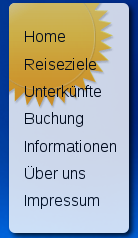
\includegraphics[scale=0.8]{screenshot_menue.png}
	\caption{Screenshot des Menü Div}
	\end{figure}
\end{frame}

\subsection{Seitenstruktur}
\begin{frame} %%Eine Folie
  \frametitle{Seitenstruktur} %%Folientitel
  \begin{block}{Seitenstruktur}
	\begin{itemize}
		\item keine Frames
		\item Div Layout
		\item Menü links
		\item Content rechts
	\end{itemize}
  \end{block}
\end{frame}


\begin{frame}
	\begin{figure}
	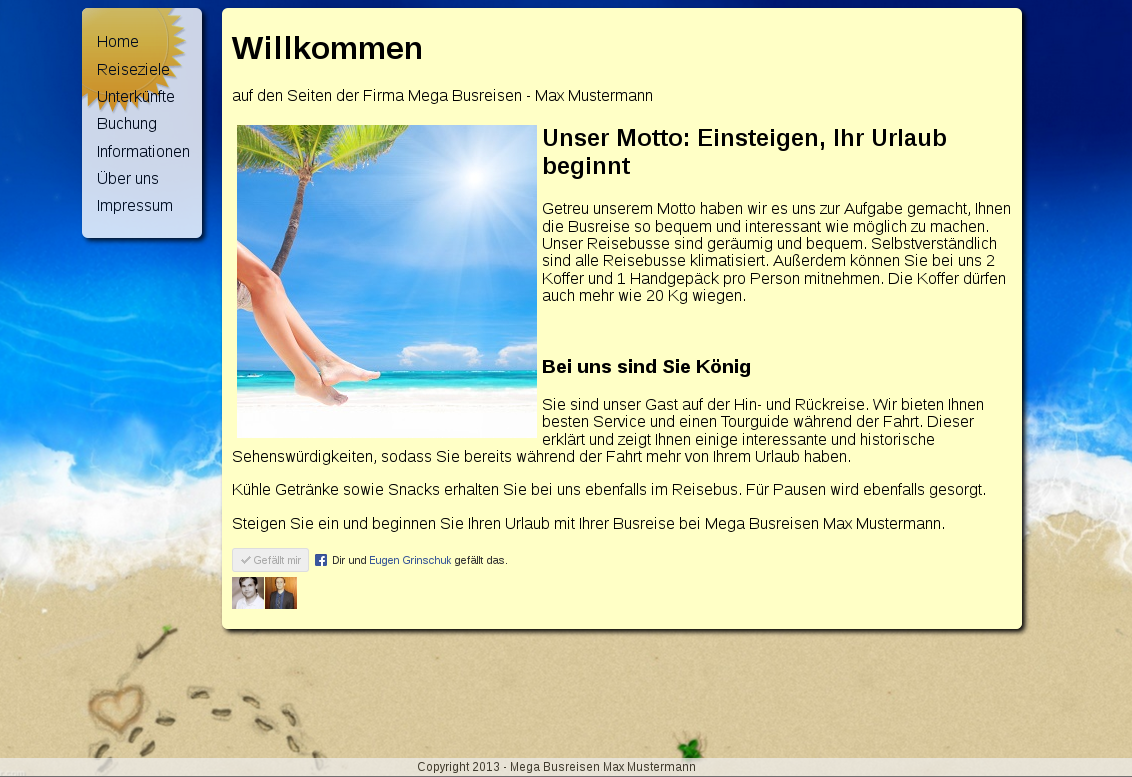
\includegraphics[scale=0.4]{screenshot_website.png}
	\caption{Screenshot \\ \tiny{\textcolor{gray}				{\url{http://www.int02-studieren-und-arbeiten.de}}}}
	\end{figure}
\end{frame}

\section{Internals}
\begin{frame} %%Eine Folie
  \frametitle{Was ist unter der Haube} %%Folientitel
	\tableofcontents[currentsection, hideothersubsections] 
\end{frame}

\subsection{PHP}
\begin{frame}[fragile]
\frametitle{PHP}

\begin{lstlisting}[language=PHP]
switch ($_GET['seite']) {

    case "reiseziele": //Reiseziele
        $site = "include/reiseziele.html";
        $title = "";
        $keywords = "";
        $description = "";
        break;
        // und weitere ...
    default: // Home Seite und alle ungueltigen Seiten
        $site = "include/inhalt.html";
        $title = "";
        $keywords = "";
        $description = "";
        break;
}

\end{lstlisting}
\end{frame}

\subsection{HTML}
\begin{frame}[fragile]
\frametitle{HTML}

\begin{lstlisting}[language=HTML]
<h1>Willkommen</h1>

<p>auf den Seiten der Firma Mega Busreisen - Max Mustermann</p>

<img src="images/reisen.jpg" alt="Reisen" title="Reisen" vspace="5" hspace="5" align="left">

<h2>Unser Motto: Einsteigen, Ihr Urlaub beginnt</h2>

<p>Getreu unserem Motto ....</p>
<br>

\end{lstlisting}
\end{frame}

\subsection{CSS}
\begin{frame}[fragile]
\frametitle{CSS}

\begin{lstlisting}[language=CSS]
body {
    background-color: white;
    font-family: Arial, Helvetica, Tahoma, sans-serif;
    font-size: 16px;
    background: url(../images/background.jpg) no-repeat center center fixed;
    background-size: cover;
}
#container {
    margin: 0px auto;
    width: 950px;
}

\end{lstlisting}
\end{frame}

\begin{frame}[fragile]
\frametitle{CSS}

\begin{lstlisting}[language=CSS, firstnumber=12]
#menu {
    float: left;
    width: 120px;
    height: 220px;
    margin-right: 20px;
    padding-top: 10px;
    background-color: #ffffff;
    box-shadow: 3px 3px 4px #000000;
    background-image:url('../images/badge_yellow.gif');
    background-repeat: no-repeat;
    background-position: -40px -40px;
    opacity: 0.8;
    border-radius: 6px;
}
\end{lstlisting}
\end{frame}

\begin{frame}[fragile]
\frametitle{CSS}

\begin{lstlisting}[language=CSS, firstnumber=51]
#inhalt {
        float: left;
        width: 780px;
        background-color: #ffffc6;
        padding: 0px 10px 20px 10px;
        margin-bottom: 20px;
        box-shadow: 3px 3px 4px #000000;
        border-radius: 6px;
}

\end{lstlisting}
\end{frame}


\subsection{JavaScript}
\begin{frame} %%Eine Folie
	\begin{figure}
	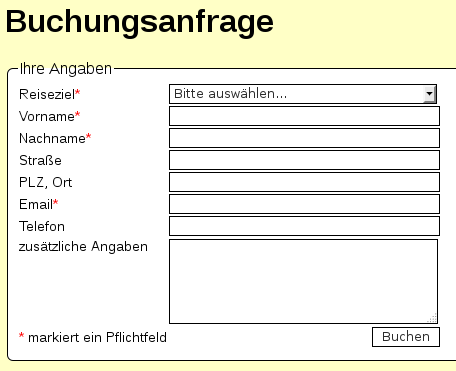
\includegraphics[scale=0.5]{screenshot_buchung.png}
	\caption{Screenshot des Buchungsformular}
	\end{figure}
\end{frame}

\begin{frame}[fragile]
\frametitle{Javascript}

\begin{lstlisting}[language=javascript]
function checkForm() {

		error = new Array();

	var reiseziel = document.getElementById('reiseziel');
	var vorname = document.getElementById('vorname');
	var nachname = document.getElementById('nachname');
	var email = document.getElementById('email');

	reiseziel.className = '';
	vorname.className = '';
	nachname.className = '';
	email.className = '';
	


\end{lstlisting}
\end{frame}

\begin{frame}[fragile]
\frametitle{Javascript}

\begin{lstlisting}[language=javascript, firstnumber=14]
	
	if (reiseziel.selectedIndex == 0) {

		reiseziel.className = 'error';
		error.push('* Reiseziel');

	}

	if (vorname.value == '') {

		vorname.className = 'error';
		error.push('* Vorname');

	}


\end{lstlisting}
\end{frame}

\begin{frame}[fragile]
\frametitle{Javascript}

\begin{lstlisting}[language=javascript, firstnumber=28]

	if (nachname.value == '') {

		nachname.className = 'error';
		error.push('* Nachname');

	}

	if (email.value == '') {

		email.className = 'error';
		error.push('* Email');

	}


\end{lstlisting}
\end{frame}

\begin{frame}[fragile]
\frametitle{Javascript}

\begin{lstlisting}[language=javascript, firstnumber=42]

	if (email.value.indexOf('@') == -1) {

		email.className = 'error';
		error.push('* keine g%FCltige Email');

	}

	if (error.length > 0) {

		var error_header = 'Folgende Pflichfelder sind nicht ausgef%FCllt:\n\n';
		alert(unescape(error_header + error.join('\n')));
		return false;
	}
	
\end{lstlisting}
\end{frame}

\begin{frame}[fragile]
\frametitle{Javascript}

\begin{lstlisting}[language=javascript, firstnumber=56]
	
	alert('Vielen Dank, Ihre Anfrage wird umgehend bearbeitet.');

}

\end{lstlisting}
\end{frame}



\subsection{Url Rewrite}
\begin{frame}[fragile]
  \frametitle{Url Rewrite}
  \framesubtitle{Apache mod\_rewrite} %%Fielenuntertitel

 \begin{block}{.htaccess}
	Suchmaschinen freundliche URL's \\
	aus index.php?seite=impressum wird impressum.html
  \end{block}

\begin{lstlisting}[language=HTML]
RewriteEngine On
RewriteBase /
RewriteRule ^(.*).html$ index.php?seite=$1
\end{lstlisting}

  \begin{block}{index.php}
	Kann Global im Code aktiviert bzw. deaktiviert werden
  \end{block}

\begin{lstlisting}[language=PHP, firstnumber=4]
define(USE_MOD_REWRITE, true);

\end{lstlisting}
\end{frame}

\subsection{Facebook}
\begin{frame}[fragile]
  \frametitle{Facebook Integration auf der Startseite}

\begin{lstlisting}[language=HTML]
<div id="fb-root"></div>
\end{lstlisting}

\begin{lstlisting}[language=JavaScript, firstnumber=3]
<script>(function(d, s, id) {
  var js, fjs = d.getElementsByTagName(s)[0];
  if (d.getElementById(id)) return;
  js = d.createElement(s); js.id = id;
  js.src = "//connect.facebook.net/de_DE/all.js#xfbml=1";
  fjs.parentNode.insertBefore(js, fjs);
}(document, 'script', 'facebook-jssdk'));</script>
\end{lstlisting}

\begin{lstlisting}[language=HTML, firstnumber=26]
<div class="fb-like" data-href="http://www.int02.studieren-und-arbeiten.de/" data-send="false" data-width="450" data-show-faces="true"></div>
\end{lstlisting}



\end{frame}


\section{Modernes Webdesign}
\begin{frame} %%Eine Folie
  \frametitle{Was zeichnet moderenes Webdesign aus?} %%Folientitel
  \begin{block}{}
	\begin{itemize}
		\item Modernes Webdesign wird mit HTML4, Javascript, PHP oder bereits mit HTML5 erstellt
		\item Moderne Webseiten werden stets mit CMS (Content Management Systemen) erstellt um die Pflege zu erleichtern
		\item Datenbanken sind beim heutigen Webseiten nahezu Pflicht
		\item Oft werden Plugins verwendet, die programmiert werden müssen oder bereits vorhanden sind
		\item Mobile Version der Webseite gehört heute nahezu dem Standard an
	\end{itemize}
  \end{block}
\end{frame}

\subsection{Ende}
\begin{frame}
	\begin{block}{}	
		\begin{center}
			Vielen Dank für Ihre Aufmerksamkeit. \\
			Fragen?
		\end{center}	
	\end{block}
	\begin{block}{Links}	
		\begin{itemize}
			\item \url{http://www.int02.studieren-und-arbeiten.de/}
			\item \url{https://github.com/derdanu/akad-int02-website}
			\item \url{https://github.com/derdanu/akad-int02-beamer}						
		\end{itemize}
	\end{block}
\end{frame}

\subsection{Quellen}
\begin{frame} %%Eine Folie
  \frametitle{Quellen} %%Folientitel
 	\begin{itemize}
		\item \url{http://www.w3.org/}
		\item \url{http://wirtschaftslexikon.gabler.de/Definition/aida-regel.html}
		\item \url{http://de.selfhtml.org/css/}
		\item \url{http://www.seo-united.de/}
		\item \url{https://support.google.com/webmasters/answer/35291?hl=de}		\item \url{http://php.net/}
 		\item \url{http://de.selfhtml.org}
		\item \url{http://openbook.galileocomputing.de/javascript_ajax/}
	\end{itemize}
\end{frame}

\begin{frame} %%Eine Folie
  \frametitle{Quellen} %%Folientitel
 	\begin{itemize}
 		\item  \url{http://www.webhelps.de/blog/2010/07/23/website-usability-checkliste/}
		\item \url{http://lehrerfortbildung-bw.de/werkstatt/websites/3benutzerfuehrung/ergonomie.htm}
		\item \url{ http://www.w3schools.com/html/html5_intro.asp}
		\item \url{http://git-scm.com/}
		\item \url{http://httpd.apache.org/docs/2.2/mod/mod_rewrite.html}
		\item \url{https://developers.facebook.com/docs/reference/plugins/like/}
	\end{itemize}
\end{frame}



\end{document}


